% best response polytope example
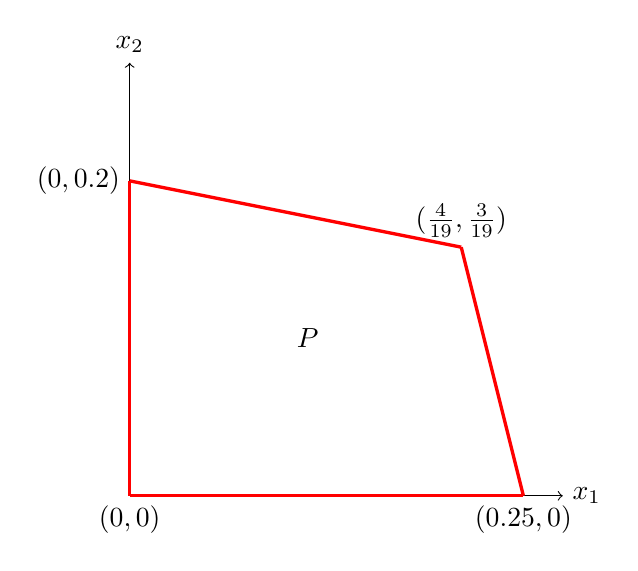
\begin{tikzpicture}
    \draw[->] (0,0) -- (5.5,0) node[right]{$x_{1}$};
    \draw[->] (0,0) -- (0,5.5) node[above]{$x_{2}$};
    \draw[red, very thick] (0,0) -- (5,0);
    \draw[red, very thick] (5,0) -- (80/19,60/19);
    \draw[red, very thick] (0,0) -- (0,4);
    \draw[red, very thick] (80/19,60/19) -- (0,4);
    \node[below] at (0,0) {$(0,0)$};
    \node[below] at (5,0) {$(0.25,0)$};
    \node[left] at (0,4) {$(0,0.2)$};
    \node[above] at (80/19,60/19) {$(\frac{4}{19}, \frac{3}{19})$};
    \node[right] at (2,2) {$P$};
\end{tikzpicture}